%%%%%%%%%%%%%%%%%%%%%%%%%%%%%%%%%%%%%%%%%%%%%%%%%
%%%%%%%%%%%%%%%%%%%%%%%%%%%%%%%%%%%%%%%%%%%%%%%%%

\chapter{Nature-based Algorithms for Prioritized Foraging}
\label{chap:third}

%%%%%%%%%%%%%%%%%%%%%%%%%%%%%%%%%%%%%%%%%%%%%%%%%
%%%%%%%%%%%%%%%%%%%%%%%%%%%%%%%%%%%%%%%%%%%%%%%%%

This chapter presents three algorithms for prioritized foraging. These three algorithms are based based upon phenomenon observed in nature. The first model is a simple foraging algorithm, called na\"ive foraging, which will form the benchmark algorithm for the experiments. Two novel swarm robotics foraging algorithms inspired by the foraging behaviour of desert ants and honey bees are also presented. Each of these algorithms have differing capabilities when it comes to memory, communication, division of labour, and navigation. The benchmark algorithm is presented in Section~\ref{naiveforaging}. Section~\ref{desertantforaging} introduces the novel foraging algorithm based on desert ants. Section~\ref{honeybeeforaging} presents a novel foraging algorithm inspired by honey bees. The algorithms are summarized in Section~\ref{prioritized:summary}.
%%%%%%%%%%%%%%%%%%%%%%%%%%%%%%%%%%%%%%%%%%%%%%%%%
%%%%%%%%%%%%%%%%%%%%%%%%%%%%%%%%%%%%%%%%%%%%%%%%%

\section{Na\"ive Foraging Algorithm}
\label{naiveforaging}

 Na\"\i ve foraging consists of the following tasks: searching for an item, grabbing an item, returning home with the item and storing the item at the sink. The steps performed by the algorithm are illustrated in Figure~\ref{naiveforagestate}.  

\begin{enumerate}
	\item Robots perform a random walk until they find an item.
	\item On locating an item, the robot grips the item. If the item has been moved before the robot is able to pick it up, the robot will continue to explore; otherwise, the robot returns the item to the correct sink using a beacon-based homing algorithm.
\end{enumerate}



\begin{figure} [h]
	\centering
	\begin{tikzpicture}[node distance=8cm]
	\node (randomwalk) [process] {random walk};
	\node (offload) [process, below of=randomwalk, yshift=4cm] {off-load};
	\node (loaditem) [process, right of=randomwalk] {load item};
	\node (homing) [process, right of=offload] {homing};
	\draw [arrow] (randomwalk) -- node[anchor=south] {locates item} (loaditem);
	\draw [arrow] (loaditem) -- node[anchor=west] {successful load} (homing);
	\draw [arrow] (homing) -- node[anchor=north] {at sink} (offload);
	\draw [arrow] (offload) -- node[anchor=west] {successful offload} (randomwalk);

	\draw[arrow,postaction={decorate,decoration={text along path,reverse path,raise=1ex,text align=center,text={unsuccessful load}}}] (loaditem) to[bend right=45] (randomwalk);
	\end{tikzpicture}
	\caption{Nai\"ve Foraging State Diagram}
	\label{foragingstatediagram}
\end{figure}

Na\"\i ve foraging includes only the most minimal set of foraging actions and is included as a baseline for comparison to evaluate how novel techniques, such as the desert-ant foraging or honey-bee foraging, compare to a standard model \cite{ostergaard2001emergent,hoff2010two}.

The following random walk is used: A robot chooses a random direction, $\sigma$, and a random distance $m\in(0,M)$ where $M$ is a chosen maximum path length. The robot walks in direction $\sigma$ for distance $m$. The robot then chooses new values for $\sigma$ and $m$. 


\section{Desert Ant Foraging}
\label{desertantforaging}


As discussed in Section~\ref{biological:ants}, due to the lack of pheromone, desert ant foraging behaviour is a very suitable model for robot foraging since no pheromone depositors or pheromone mimickry is required. Instead of pheromone, desert ants use path integration (PI) to memorize the location of an existing food source and later to return to the memorized source to find more food, which was also addressed in Section~\ref{biological:ants}. The notion of returning to a previously explored site is known as site fidelity \cite{switzer1993site}. The desert ant algorithm does not require communication between robots or the dispersal of beacons, and is thus simpler than other many swarm robotics foraging algorithms. The desert ant foraging robots can be in the following states:

\begin{enumerate}
	\item\textbf{Exploration State} -- A robot in the exploration state performs a random walk with PI. The random walk used was the same as discussed in Section~\ref{naiveforaging}. The purpose of the exploration state is to explore the environment to locate items. 
	\item\textbf{Loading State} -- On finding an item, the robot switches into the loading state. In the loading state, the robot loads the item and memorizes the current PI vector. The PI vector is memorized so that the robot can use the it to return to the sink and then later to return the site where the item was found. If loading the item fails (perhaps due to another robot loading the item), then the robot returns to the exploration state; else the robot moves into the homing state.
	\item\textbf{Homing State} -- In the homing state, the robot uses the PI vector to move to the sink. The use of the PI vector will enable the robot to follow the most direct route back to the sink.
	\item\textbf{Offloading State} -- When the robot arrives at the sink, the robot switches into the offloading state where the robot simply offloads the item into the sink. 
	\item\textbf{Locating State} -- Once the robot has offloaded the item, the robot switches to the locating state. In the locating state, the robot follows the memorized PI vector to the location of the previous item. The premise of returning to the site where the previous item was found is that more items may exist where the previous item was located in order to locate more items. If another item is found, the robot moves into the loading state; otherwise the robot returns to the exploration state in the search of new items. 
\end{enumerate}

All robots begin at random positions adjacent to the sink in the exploration state. The desert ant foraging states and transitions are illustrated in Figure~\ref{fig:desertantstate}.

\begin{figure} [h]
	\centering
	\begin{tikzpicture}[node distance=6cm]
	\node (explorationstate) [process] {explore};
	\node (loadstate) [process, right of=randomwalk] {loading};
	\node (homing) [process, below of=loadstate,yshift=2cm] {homing};
	\node (offload) [process, left of=homing] {offload};
	\node (locating) [process, left of=explorationstate] {locating};
	\draw [arrow] (explorationstate) -- node[anchor=south] {locates item} (loadstate);
	\draw [arrow] (loadstate) -- node[anchor=west] {successful load} (homing);
	\draw [arrow] (homing) -- node[anchor=south] {at sink} (offload);
	\draw [arrow] (offload) -- node[anchor=east] {offload complete} (locating);
	\draw [arrow] (locating) -- node[anchor=south] {item not found} (explorationstate);
	\draw[arrow,postaction={decorate,decoration={text along path,raise=1ex,text align=center,text={locates item}}}] (locating) to[bend left=45] (loadstate);
	\draw[arrow,postaction={decorate,decoration={text along path,reverse path, raise=1ex,text align=center,text={unsuccessful load}}}] (loadstate) to[bend left=45] (explorationstate);
	\end{tikzpicture}
	\caption{Desert Ant Foraging State Diagram}
	\label{fig:desertantstate}
\end{figure}

	
%%%%%%%%%%%%%%%%%%%%%%%%%%%%%%%%%%%%%%%%%%%%%%%%%
%%%%%%%%%%%%%%%%%%%%%%%%%%%%%%%%%%%%%%%%%%%%%%%%%

\section{Honey Bee Foraging}
\label{honeybeeforaging}
%TODO Describe the 3 states referring back to where they were discussed in the previous section.

The honey bee priotizied foraging algorithm presented in this section is based on the mathematical model of honey bee foraging in \cite{seeley2009wisdom}. A portion of the robots are initialized as scouts and the rest  as unemployed foragers in a waiting state. All robots are initialized adjacent to the item sinks.

Fig \ref{honeybeestate} provides a simplified state diagram for the honey bee prioritized foraging algorithm. State transitions are described as follows: 

\begin{enumerate}

\item Each scout robot performs a random walk. The random walk used is the same as discussed in Section~\ref{naiveforaging}. Upon finding an item $\vartheta$ at site $\xi$, the robot loads the item and then performs an evaluation of the quality of the site $\xi$. The site quality is denoted by $\mu$. Before returning to the sink, the scout memorizes the PI vector $v$. Using PI vector $v$, The scout then returns the item $u$ to the sink, resulting in the most direct route to the sink.  When the scout robot has returned to the sink and successfully offloaded the item, the scout robot switches into the recruitment state.

\item In the recruitment state, the scout robot will decide whether to communicate the location, $v$ and quality $\mu$, of the previous site $\xi$, to the unemployed workers at the sink. The communication is akin to the dance performed by honey bees in nature, as discussed in Section~\ref{honeybeeinnature}. A scout robot's ``dance" takes the form of broadcast communication between the scout and the unemployed forager robots at sink $S$.

The scout robot will examine the site quality, $\mu$, to decide whether to communicate the details of site $\xi$. If the estimated quality of the site, $\mu$, is less than the dance threshold, $\phi$, the scout robot does not communicate the site details and instead returns to foraging state. If $\mu$, is greater or equal to $\phi$, the scout robot will communicate the site quality and location for the unemployed foragers.

\item After the scout robot has completed the recruitment step, the scout robot must decide to either stay a scout and switch back to the exploration state or become a forager and begin foraging the previous site. The scout robot generates a random variable, $r\in(0,1)$. If $r$ is less than a division of labour control parameter, $\rho$, then the scout robot remains a scout and begins to explore the environment. If A$r$ is greater than or equal to $\rho$ then the scout becomes a forager and begins to location the prior site

\item Each unemployed forager chooses, with a probability $\alpha$, to be recruited by a broadcasting scout robot. If a unemployed forager robot are recruited by the scout robot, the unemployed forager robot becomes an employed forager robot in the locating state, else the unemployed forager robot stays in the waiting state.

\item An employed forager robot becomes an unemployed forager robot, when the foraging site that the scout broadcasted has been depleted. A foraging site has been depleted when a employed forager robot can't detect an item in the area surrounding location $v$.

\item Unemployed foragers become scout robots, if no scout robot broadcasts are detected for $t_{max}$ time steps. The control parameter $t_{max}$ 
is the maximum waiting time an unemployed forager can spend in the waiting state, before switching to a scout robot. Decreasing $t_{max}$ results in more scout robots exploring the environment and less unemployed foragers that a scout robot, who may have found quality sites, can recruit. Increasing $t_{max}$ results in a greater quantity of unemployed foragers. The greater quantity of unemployed foragers can form a large work force for a recruiting scout, however too many unemployed foragers results in a smaller workforce in the foraging environment.
\end{enumerate}

\begin{figure}[h]
	\centering
	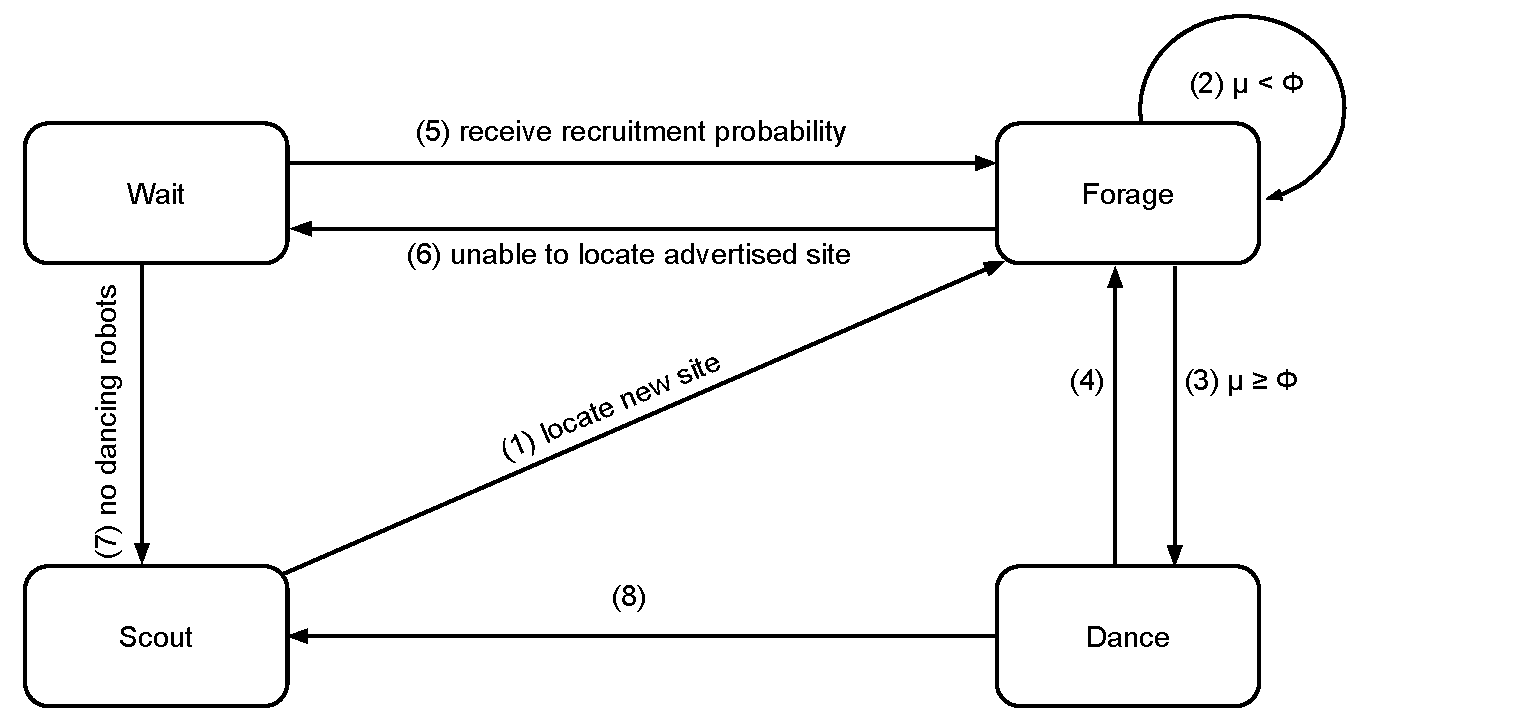
\includegraphics[width=\textwidth]{chapters/chapter3/figures/HoneyBee.pdf}
	\caption{Honey Bee Foraging State Diagram }
	\label{honeybeestate}
\end{figure}

The quality, $\mu_t$, of site $\xi$, for a robot scouting items of type $t$ is calculated as the estimated density of items of type $t$ in the local vicinity of the found item. The robot has distance sensor values $k_i\in[0,1]$ for $ i = 1...n$ where $n$ is the number of distance sensors. A distance sensor reading of 0 means that nothing is detected in the sensor's range and a distance sensor reading of 1 indicates that the robot is touching an item. The sensor value $k_i$, for item type $t$, denoted $k_{i_t}$, is calculated using 
\begin{equation}
\label{densitytype}
k_{i_t}=
    \begin{cases}
      k_i & \text{if item $i$ is type $t$} \\
      0 & \text{otherwise}
    \end{cases}
\end{equation}

The site quality of type $t$, $\mu_t$, is calculated using
\begin{equation}
\label{density}
\mu_t = \frac{1}{n}\sum\limits_{i=1}^n k_{i_t}
\end{equation}
where 

In nature, in times of drought, bees prioritize water over nectar or pollen. Bees are sent out to forage water; however, if they happen to encounter pollen, they will forage the pollen but will not communicate the discovery of the pollen site to the unemployed foragers  \cite{seeley2009wisdom}. Using the bee's priorization of resources as inspiration, an item-type division of labout is introduced. Item-type division of labout is defined in this thesis as the division of labour between foraging prioritized item types and non-prioritized item types.
The rules for item-type division of labour are based on the behaviour of bees under environmental pressure, as follows:

\begin{enumerate}
\item A robot foraging the prioritized type will forage a non-prioritized type only if a prioritized item can not be located for the maximum time period, $f_{max}$.
\item A robot foraging the non-prioritized item type will forage the non-prioritized item type until the robot fails to relocate a previously located non-prioritized item type site or until the robot locates a prioritized item. In either case, the robot will switch to foraging the prioritized item type.
\item A robot foraging a non-prioritized item will not communicate the location of the non-prioritized item site by dancing. 
\end{enumerate}

To more succinctly and specifically define the honey bee prioritized foraging algorithm, the algorithm pseudo code for each behaviour has been provided: Exploration state of a scout robot is outlined in Algorithm~\ref{algorithm:explore}. Algorithm~\ref{algorithm:scout:homing} explains the homing behaviour of a scout robot while the recruitment state of a scout robot is defined in Algorithm~\ref{algorithm:recruit}. 

For the purpose of this study, all swarms are given an initial item type to forage. The robots of desert ant foraging algorithm and the na\"ive algorithm do not have item-type level division of labour and thus will continue to forage the same item-type throughout the experiments. The robots in the honey bee algorithm may switch what item-types they forage during the experiment, due to the item-type division of labour. The presented algorithms differ in three main properties as summarized in Table \ref{properties}.

\begin{algorithm}
\caption{Explore State (Scout)}
\label{algorithm:explore}
\begin{algorithmic}[1]
\Function{explore}{state}
\State \Call{move}{random\_direction}
\State \Call{update}{\={v}}
\If {\Call{find}{item,division}}
 	\State \Call{estimate\_site\_density}{ }
	\State $destination \gets v$
	\State \Call{load}{item}
\ElsIf {$i > f_{max}$ and $i < t_{max}$}
	\State $division \gets WASTE$
\ElsIf {$i > t_{max}$}
	\State $state \gets HOMING$
\EndIf
\State $i =i + 1$
\EndFunction
\end{algorithmic}
\end{algorithm}

\begin{algorithm}
\caption{Homing State (Employed Forager)}
\label{algorithm:employedforager:homing}
\begin{algorithmic}[1]
\Function{forage-homing}{state}
\State $direction = \Call{calc\_dir\_to}{home,v}$
\State \Call{move}{direction}
\If {\Call{at}{home}}
	\State{$state \gets OFFLOAD$}
\EndIf
\State $i =i + 1$
\EndFunction
\end{algorithmic}
\end{algorithm}

\begin{algorithm}
\caption{Recruit State (Scout)}
\label{algorithm:recruit}
\begin{algorithmic}[1]
\Function{recruit}{state}
\If {$i < t_{max}$}
	\State \Call{broadcast}{ destination } 
\Else 
	\If {$random < \rho$} 
		\Comment{recruit self}
		\State{$state \gets FORAGING$}
	\Else
		\State{$state \gets EXPLORING$}
	\EndIf
\EndIf
\State $i =i + 1$
\EndFunction
\end{algorithmic}
\end{algorithm}

\begin{algorithm}
\caption{Homing State (Scout)}
\label{algorithm:scout:homing}
\begin{algorithmic}[1]
\Function{explore homing}{state}
\If{$i == 0$}
	\State{$destination \gets v$}
	
\EndIf
\State{$direction \gets \Call{calc\_dir\_to}{destination, v}$}
\If{\Call{is\_valid\_move}{direction}}
	\State \Call{move}{direction}
	\If {\Call{at}{home}}
		\State $state \gets UNLOADING$
	\Else
		\State $state \gets BEACON-HOMING$	
	\EndIf
\EndIf
\State $i =i + 1$
\EndFunction
\end{algorithmic}
\end{algorithm}

\begin{algorithm}
\caption{Unloading State (Employed Forager)}
\label{algorithm:employedforager:unloading}
\begin{algorithmic}[1]
\Function{unloading}{state}
	\If {\Call{is}{loaded}}
		\State \Call{offload}{ }
		\If{$\mu > \phi$}
			\State $state \gets RECRUIT$
		\Else
			\State $state \gets LOCATING$
		\EndIf
	\Else
		\State $state \gets SINK-AVOIDANCE$ \Comment{ie waiting}
	\EndIf
	\State $i =i + 1$
\EndFunction

\end{algorithmic}
\end{algorithm}

\begin{algorithm}
\caption{Locating State (Employed Forager)}
\label{algorithm:employedforager:locating}
\begin{algorithmic}[1]
\Function{locating}{state}
	\If {$i==0$}
		\State $destination \gets broadcast - location$
	\EndIf
	\State \Call{calc\_dir\_to}{destination, v}
	\State \Call{move}{direction}
	\If {\Call{at}{destination,v}}
		\State $state \gets LOADING$
	\ElsIf {\Call{see}{item}}
		\State $state \gets LOADING$
	\ElsIf {\Call{wall\_collision}{ }}
		\Comment{not sure if this is right}
		\State{$state \gets LOADING$}
	\EndIf
	\State $i =i + 1$
\EndFunction
\end{algorithmic}
\end{algorithm}

\begin{algorithm}
\caption{Sink Avoidance State (Employed Forager)}
\label{algorithm:sinkavoidance}
\begin{algorithmic}[1]
\Function{sink avoidance}{state}
\If { $\Call{count}{robots, camera} > 1$}
	\State $direction \gets \Call{get\_clearest\_direction}{ }$ \Comment{using desirability - expand on}
	\State \Call{move}{direction}
\Else
	\State $state \gets WAITING$
\EndIf
\State $i =i + 1$
\EndFunction
\end{algorithmic}
\end{algorithm}
\begin{algorithm}
\caption{Waiting State (Unemployed Forager)}
\label{algorithm:unemployedforager:locating}
\begin{algorithmic}[1]
\Function{waiting}{state}
\If {$i == 0$}
	\State \Call{reset}{v} 
\ElsIf {$i > \phi$} \Comment{max waiting reps?}
	\State{$state \gets EXPLORING$}
\Else
	\State \Call{listen}{ }
\EndIf
\State $i =i + 1$
\EndFunction
\end{algorithmic}
\end{algorithm}

\begin{algorithm}
\caption{Beacon homing state}
\label{algorithm:beaconhoming}
\begin{algorithmic}[1]
\Function{beacon homing}{}
\If {\Call{at}{destination}}
	\State $state \gets RECRUITING$
\EndIf
\State $direction \gets \Call{calc\_dir\_to}{homing\_beacon}$
\State \Call{move}{direction}
\State $i =i + 1$
\EndFunction
\end{algorithmic}
\end{algorithm}

\begin{algorithm}
\caption{Loading State (Employed Forager)}
\label{algorithm:loading}
\begin{algorithmic}[1]
\Function{loading}{state}
\If {\Call{identify}{item}}
	\State \Call{load}{item}
	\State{$state \gets HOMING$}
\Else
	\State{$state \gets LOCAL\_CLUSTER\_SEARCH$}
\EndIf
\EndFunction
\end{algorithmic}
\end{algorithm}

\begin{algorithm}
\caption{Local Cluster Search State (Employed Forager)}
\label{algorithm:employedforager:localclustersearch}
\begin{algorithmic}[1]
\Function{local\_cluster\_search}{state}
\If {$c < max\_search\_range$}
	\If {\Call{identify}{item} and \Call{loadable}{ }}
		\State \Call{load\_item}{ }
		\State $density \gets \Call{estimate\_area\_density}{ }$
		\State{$state \gets HOMING$}	
	\ElsIf {\Call{identify}{item} and \textbf{not} \Call{loadable}{ }}
		\State $direction \gets \Call{calc\_dir\_to}{item}$
		\State \Call{move}{direction}
	\Else
		\State \Call{move}{random\_direction}	
	\EndIf
\Else
	\State{$state \gets HOMING$}
\EndIf
\State $i =i + 1$
\EndFunction
\end{algorithmic}
\end{algorithm}


\section{Summary}
\label{prioritized:summary}

This chapter introduced two novel algorithms for foraging robot swarms: a desert ant inspired foraging algorithm, as well as a honey bee inspired foraging algorithm. A benchmark algorithm going by the name na\"ive foraging, is also presented. Probabilistic state machines are presented for each algorithm and the algorithms are discussed in terms of their memory, communication and division of labour capabilities. An overview of the properties of the algorithms can be seen in Table \ref{properties}.

\begin{table} [h]
    \caption{Properties of the foraging algorithms used in this study}
    \label{properties}
	\centering
    \begin{tabular}{|l|c c c|} \hline
    Property           & Na\"ive  & Desert Ant  & Honey Bee  \\ \hline
    Memory             & \xmark  & \cmark     & \cmark    \\
    Communication      & \xmark  & \xmark     & \cmark    \\
    Division of Labour & \xmark  & \xmark     & \cmark    \\ \hline
    \end{tabular}

\end{table}


%%%%%%%%%%%%%%%%%%%%%%%%%%%%%%%%%%%%%%%%%%%%%%%%%
%%%%%%%%%%%%%%%%%%%%%%%%%%%%%%%%%%%%%%%%%%%%%%%%%